\documentclass[20pt,-letter paper]{article}
\usepackage{amsmath}
\usepackage{gensymb}
\usepackage{mathtools}
\providecommand{\brak}[1]{\ensuremath{\left(#1\right)}}
\title{}
%\author{Prof.G V V sharma}
\date{\today}

\begin{document}

\maketitle{question}

\begin{enumerate}

\item In the cricult shift, the initial binary content of the shift register A $1101$ and that of shift register B is $1010$ The shift registers are positive edge triggered, and the gates have no delay.

when the shift control is high,what will be the binary content of the shift registers $A$ and $B$ after clock pulses ?


\begin {figure}[h]
 \centering
 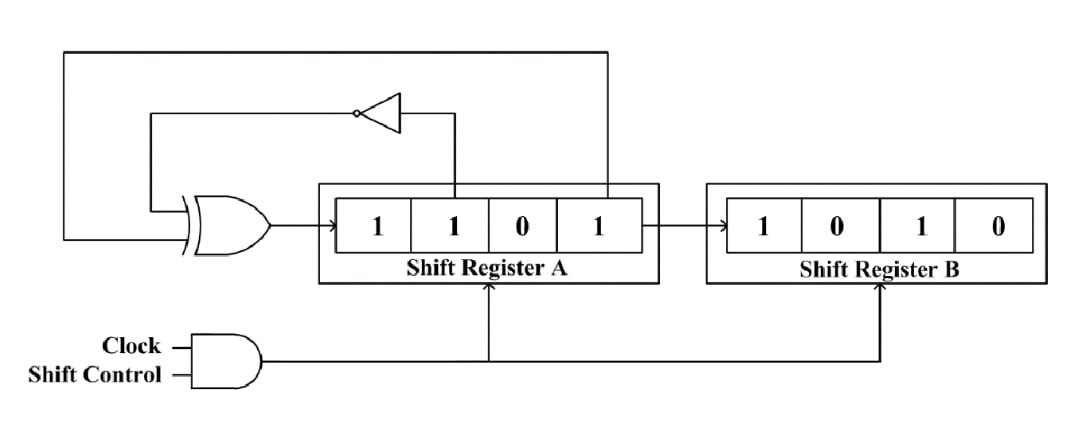
\includegraphics[width=1.0\textwidth]{/sdcard/Download/termux/Gate.jpg}
\end{figure}

\begin{enumerate}
\item $A= 1101,B=1101$
\item $A=1110 ,B=1001$
\item $A=0101 ,B=1101$
\item $A=1010 ,B=1111$
\end {enumerate}
\end {enumerate}
\end {document}
